\documentclass{article}
\usepackage{lmodern}
\usepackage[T1]{fontenc}
\usepackage{shapepar}
\usepackage{microtype}
\usepackage{lipsum}
\usepackage{pgfplots}
\pgfplotsset{compat=1.9}
\usepackage{tikz}
\usetikzlibrary{calc,fit,intersections,folding}
\usepackage{pstricks-add}
\usetikzlibrary{arrows.meta,angles,arrows,quotes,backgrounds,calc}

\usepackage[left = 5mm, right = 5mm]{geometry}

\newcommand{\clrone}{blue}
\newcommand{\clrtwo}{red}

\begin{document}
\thispagestyle{empty}

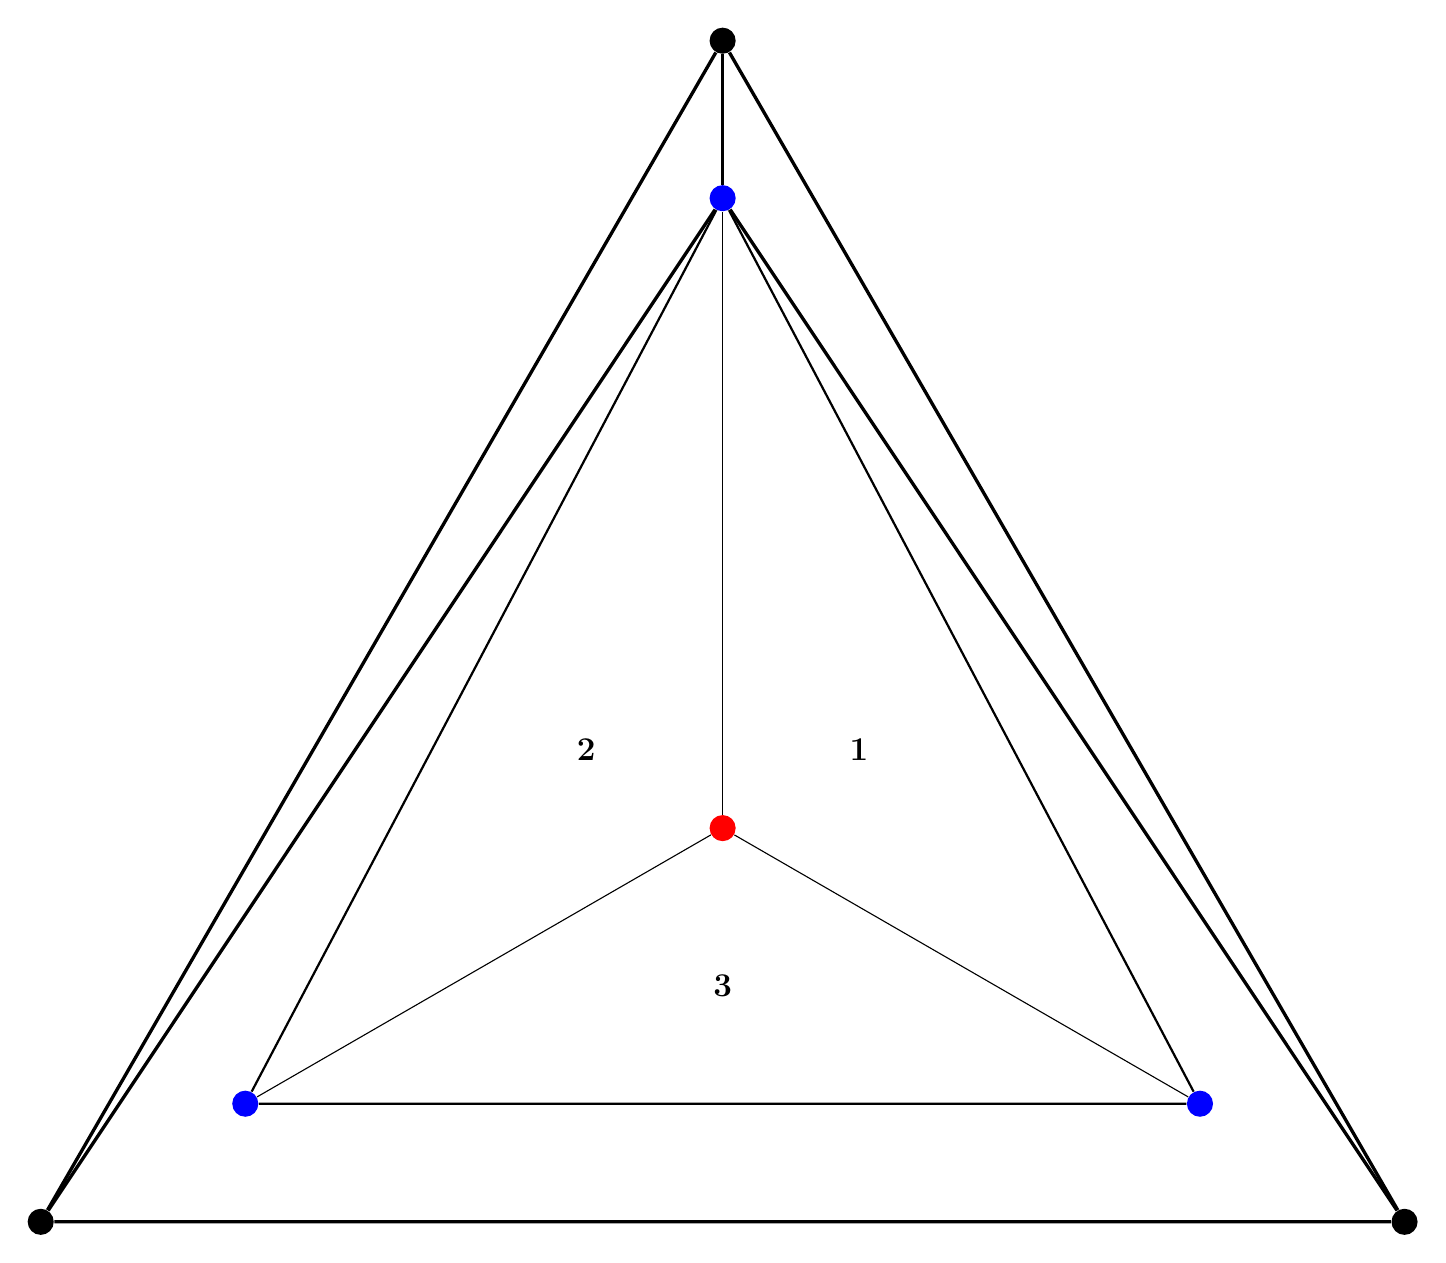
\begin{tikzpicture}[scale = 2]
    \foreach \angle in {0,...,2} {
        \node[fill, circle] (shell\angle) at (90+\angle*120:5) {};
    }
    \draw[very thick] (shell0) -- (shell1) -- (shell2) -- (shell0);

    \node[fill, circle, \clrone] (layer1t) at (90:4) {};
    \foreach\i in {0,1,2} {
        \draw[very thick] (layer1t) -- (shell\i);
    }

    \node[fill, circle, \clrone] (layer1l) at (90+120:3.5) {};
    \node[fill, circle, \clrone] (layer1r) at (90+240:3.5) {};
    \draw[thick] (layer1t) -- (layer1l) -- (layer1r) -- (layer1t);

    \node[fill, circle, \clrtwo] (layer2) at (0,0) {};
    \foreach\i in {t,l,r} {
        \draw (layer2) -- (layer1\i);
    }
    \node at (30:1) {\large\bf 1};
    \node at (30+120:1) {\large\bf 2};
    \node at (30+240:1) {\large\bf 3};
\end{tikzpicture}    

\end{document}